\documentclass[1p]{elsarticle_modified}
%\bibliographystyle{elsarticle-num}

%\usepackage[colorlinks]{hyperref}
%\usepackage{abbrmath_seonhwa} %\Abb, \Ascr, \Acal ,\Abf, \Afrak
\usepackage{amsfonts}
\usepackage{amssymb}
\usepackage{amsmath}
\usepackage{amsthm}
\usepackage{scalefnt}
\usepackage{amsbsy}
\usepackage{kotex}
\usepackage{caption}
\usepackage{subfig}
\usepackage{color}
\usepackage{graphicx}
\usepackage{xcolor} %% white, black, red, green, blue, cyan, magenta, yellow
\usepackage{float}
\usepackage{setspace}
\usepackage{hyperref}

\usepackage{tikz}
\usetikzlibrary{arrows}

\usepackage{multirow}
\usepackage{array} % fixed length table
\usepackage{hhline}

%%%%%%%%%%%%%%%%%%%%%
\makeatletter
\renewcommand*\env@matrix[1][\arraystretch]{%
	\edef\arraystretch{#1}%
	\hskip -\arraycolsep
	\let\@ifnextchar\new@ifnextchar
	\array{*\c@MaxMatrixCols c}}
\makeatother %https://tex.stackexchange.com/questions/14071/how-can-i-increase-the-line-spacing-in-a-matrix
%%%%%%%%%%%%%%%

\usepackage[normalem]{ulem}

\newcommand{\msout}[1]{\ifmmode\text{\sout{\ensuremath{#1}}}\else\sout{#1}\fi}
%SOURCE: \msout is \stkout macro in https://tex.stackexchange.com/questions/20609/strikeout-in-math-mode

\newcommand{\cancel}[1]{
	\ifmmode
	{\color{red}\msout{#1}}
	\else
	{\color{red}\sout{#1}}
	\fi
}

\newcommand{\add}[1]{
	{\color{blue}\uwave{#1}}
}

\newcommand{\replace}[2]{
	\ifmmode
	{\color{red}\msout{#1}}{\color{blue}\uwave{#2}}
	\else
	{\color{red}\sout{#1}}{\color{blue}\uwave{#2}}
	\fi
}

\newcommand{\Sol}{\mathcal{S}} %segment
\newcommand{\D}{D} %diagram
\newcommand{\A}{\mathcal{A}} %arc


%%%%%%%%%%%%%%%%%%%%%%%%%%%%%5 test

\def\sl{\operatorname{\textup{SL}}(2,\Cbb)}
\def\psl{\operatorname{\textup{PSL}}(2,\Cbb)}
\def\quan{\mkern 1mu \triangleright \mkern 1mu}

\theoremstyle{definition}
\newtheorem{thm}{Theorem}[section]
\newtheorem{prop}[thm]{Proposition}
\newtheorem{lem}[thm]{Lemma}
\newtheorem{ques}[thm]{Question}
\newtheorem{cor}[thm]{Corollary}
\newtheorem{defn}[thm]{Definition}
\newtheorem{exam}[thm]{Example}
\newtheorem{rmk}[thm]{Remark}
\newtheorem{alg}[thm]{Algorithm}

\newcommand{\I}{\sqrt{-1}}
\begin{document}

%\begin{frontmatter}
%
%\title{Boundary parabolic representations of knots up to 8 crossings}
%
%%% Group authors per affiliation:
%\author{Yunhi Cho} 
%\address{Department of Mathematics, University of Seoul, Seoul, Korea}
%\ead{yhcho@uos.ac.kr}
%
%
%\author{Seonhwa Kim} %\fnref{s_kim}}
%\address{Center for Geometry and Physics, Institute for Basic Science, Pohang, 37673, Korea}
%\ead{ryeona17@ibs.re.kr}
%
%\author{Hyuk Kim}
%\address{Department of Mathematical Sciences, Seoul National University, Seoul 08826, Korea}
%\ead{hyukkim@snu.ac.kr}
%
%\author{Seokbeom Yoon}
%\address{Department of Mathematical Sciences, Seoul National University, Seoul, 08826,  Korea}
%\ead{sbyoon15@snu.ac.kr}
%
%\begin{abstract}
%We find all boundary parabolic representation of knots up to 8 crossings.
%
%\end{abstract}
%\begin{keyword}
%    \MSC[2010] 57M25 
%\end{keyword}
%
%\end{frontmatter}

%\linenumbers
%\tableofcontents
%
\newcommand\colored[1]{\textcolor{white}{\rule[-0.35ex]{0.8em}{1.4ex}}\kern-0.8em\color{red} #1}%
%\newcommand\colored[1]{\textcolor{white}{ #1}\kern-2.17ex	\textcolor{white}{ #1}\kern-1.81ex	\textcolor{white}{ #1}\kern-2.15ex\color{red}#1	}

{\Large $\underline{10_{78}~(K10a_{17})}$}

\setlength{\tabcolsep}{10pt}
\renewcommand{\arraystretch}{1.6}
\vspace{1cm}\begin{tabular}{m{100pt}>{\centering\arraybackslash}m{274pt}}
\multirow{5}{120pt}{
	\centering
	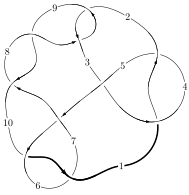
\includegraphics[width=112pt]{../../../GIT/diagram.site/Diagrams/png/162_10_78.png}\\
\ \ \ A knot diagram\footnotemark}&
\allowdisplaybreaks
\textbf{Linearized knot diagam} \\
\cline{2-2}
 &
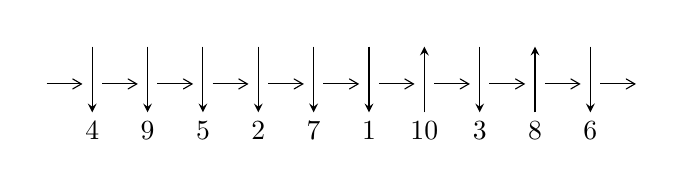
\begin{tikzpicture}[x=20pt, y=17pt]
	% nodes
	\node (C0) at (0, 0) {};
	\node (C1) at (1, 0) {};
	\node (C1U) at (1, +1) {};
	\node (C1D) at (1, -1) {4};

	\node (C2) at (2, 0) {};
	\node (C2U) at (2, +1) {};
	\node (C2D) at (2, -1) {9};

	\node (C3) at (3, 0) {};
	\node (C3U) at (3, +1) {};
	\node (C3D) at (3, -1) {5};

	\node (C4) at (4, 0) {};
	\node (C4U) at (4, +1) {};
	\node (C4D) at (4, -1) {2};

	\node (C5) at (5, 0) {};
	\node (C5U) at (5, +1) {};
	\node (C5D) at (5, -1) {7};

	\node (C6) at (6, 0) {};
	\node (C6U) at (6, +1) {};
	\node (C6D) at (6, -1) {1};

	\node (C7) at (7, 0) {};
	\node (C7U) at (7, +1) {};
	\node (C7D) at (7, -1) {10};

	\node (C8) at (8, 0) {};
	\node (C8U) at (8, +1) {};
	\node (C8D) at (8, -1) {3};

	\node (C9) at (9, 0) {};
	\node (C9U) at (9, +1) {};
	\node (C9D) at (9, -1) {8};

	\node (C10) at (10, 0) {};
	\node (C10U) at (10, +1) {};
	\node (C10D) at (10, -1) {6};
	\node (C11) at (11, 0) {};

	% arrows
	\draw[->,>={angle 60}]
	(C0) edge (C1) (C1) edge (C2) (C2) edge (C3) (C3) edge (C4) (C4) edge (C5) (C5) edge (C6) (C6) edge (C7) (C7) edge (C8) (C8) edge (C9) (C9) edge (C10) (C10) edge (C11) ;	\draw[->,>=stealth]
	(C1U) edge (C1D) (C2U) edge (C2D) (C3U) edge (C3D) (C4U) edge (C4D) (C5U) edge (C5D) (C6U) edge (C6D) (C7D) edge (C7U) (C8U) edge (C8D) (C9D) edge (C9U) (C10U) edge (C10D) ;
	\end{tikzpicture} \\
\hhline{~~} \\& 
\textbf{Solving Sequence} \\ \cline{2-2} 
 &
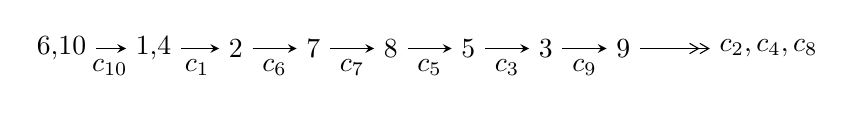
\begin{tikzpicture}[x=28pt, y=7pt]
	% node
	\node (A0) at (-1/8, 0) {6,10};
	\node (A1) at (17/16, 0) {1,4};
	\node (A2) at (17/8, 0) {2};
	\node (A3) at (25/8, 0) {7};
	\node (A4) at (33/8, 0) {8};
	\node (A5) at (41/8, 0) {5};
	\node (A6) at (49/8, 0) {3};
	\node (A7) at (57/8, 0) {9};
	\node (C1) at (1/2, -1) {$c_{10}$};
	\node (C2) at (13/8, -1) {$c_{1}$};
	\node (C3) at (21/8, -1) {$c_{6}$};
	\node (C4) at (29/8, -1) {$c_{7}$};
	\node (C5) at (37/8, -1) {$c_{5}$};
	\node (C6) at (45/8, -1) {$c_{3}$};
	\node (C7) at (53/8, -1) {$c_{9}$};
	\node (A8) at (9, 0) {$c_{2},c_{4},c_{8}$};

	% edge
	\draw[->,>=stealth]	
	(A0) edge (A1) (A1) edge (A2) (A2) edge (A3) (A3) edge (A4) (A4) edge (A5) (A5) edge (A6) (A6) edge (A7) ;
	\draw[->>,>={angle 60}]	
	(A7) edge (A8);
\end{tikzpicture} \\ 

\end{tabular} \\

\footnotetext{
The image of knot diagram is generated by the software ``\textbf{Draw programme}" developed by Andrew Bartholomew(\url{http://www.layer8.co.uk/maths/draw/index.htm\#Running-draw}), where we modified some parts for our purpose(\url{https://github.com/CATsTAILs/LinksPainter}).
}\phantom \\ \newline 
\centering \textbf{Ideals for irreducible components\footnotemark of $X_{\text{par}}$} 
 
\begin{align*}
I^u_{1}&=\langle 
- u^{11}- u^{10}+2 u^9+3 u^8-2 u^7-4 u^6-2 u^5+u^4+2 u^3+u^2+b- u-1,\\
\phantom{I^u_{1}}&\phantom{= \langle  }- u^{11}- u^{10}+2 u^9+3 u^8-2 u^7-4 u^6-2 u^5+u^4+u^3+u^2+a- u-1,\\
\phantom{I^u_{1}}&\phantom{= \langle  }u^{13}+u^{12}-3 u^{11}-4 u^{10}+4 u^9+7 u^8-5 u^6-3 u^5+3 u^3+2 u^2-1\rangle \\
I^u_{2}&=\langle 
u^{20}-6 u^{18}+\cdots+b-2 u,\;2 u^{21}+u^{20}+\cdots+a+1,\;u^{22}+u^{21}+\cdots-4 u^2+1\rangle \\
I^u_{3}&=\langle 
b+1,\;a+2,\;u+1\rangle \\
\\
\end{align*}
\raggedright * 3 irreducible components of $\dim_{\mathbb{C}}=0$, with total 36 representations.\\
\footnotetext{All coefficients of polynomials are rational numbers. But the coefficients are sometimes approximated in decimal forms when there is not enough margin.}
\newpage
\renewcommand{\arraystretch}{1}
\centering \section*{I. $I^u_{1}= \langle - u^{11}- u^{10}+\cdots+b-1,\;- u^{11}- u^{10}+\cdots+a-1,\;u^{13}+u^{12}+\cdots+2 u^2-1 \rangle$}
\flushleft \textbf{(i) Arc colorings}\\
\begin{tabular}{m{7pt} m{180pt} m{7pt} m{180pt} }
\flushright $a_{6}=$&$\begin{pmatrix}0\\u\end{pmatrix}$ \\
\flushright $a_{10}=$&$\begin{pmatrix}1\\0\end{pmatrix}$ \\
\flushright $a_{1}=$&$\begin{pmatrix}1\\u^2\end{pmatrix}$ \\
\flushright $a_{4}=$&$\begin{pmatrix}u^{11}+u^{10}-2 u^9-3 u^8+2 u^7+4 u^6+2 u^5- u^4- u^3- u^2+u+1\\u^{11}+u^{10}-2 u^9-3 u^8+2 u^7+4 u^6+2 u^5- u^4-2 u^3- u^2+u+1\end{pmatrix}$ \\
\flushright $a_{2}=$&$\begin{pmatrix}u^{12}+u^{11}-2 u^{10}-3 u^9+2 u^8+4 u^7+2 u^6- u^5- u^4- u^3+u^2+u+1\\u^{12}+u^{11}-2 u^{10}-3 u^9+2 u^8+4 u^7+2 u^6- u^5-2 u^4- u^3+2 u^2+u\end{pmatrix}$ \\
\flushright $a_{7}=$&$\begin{pmatrix}- u\\- u^3+u\end{pmatrix}$ \\
\flushright $a_{8}=$&$\begin{pmatrix}- u^3\\- u^3+u\end{pmatrix}$ \\
\flushright $a_{5}=$&$\begin{pmatrix}u^3\\u^5- u^3+u\end{pmatrix}$ \\
\flushright $a_{3}=$&$\begin{pmatrix}u^{11}+u^{10}-2 u^9-3 u^8+2 u^7+4 u^6+u^5- u^4- u^3- u^2+u+1\\u^{11}+u^{10}-2 u^9-3 u^8+u^7+4 u^6+3 u^5- u^4-3 u^3- u^2+u+1\end{pmatrix}$ \\
\flushright $a_{9}=$&$\begin{pmatrix}u^6- u^4+1\\u^6-2 u^4+u^2\end{pmatrix}$\\&\end{tabular}
\flushleft \textbf{(ii) Obstruction class $= -1$}\\~\\
\flushleft \textbf{(iii) Cusp Shapes $= -2 u^{11}+2 u^{10}+8 u^9-2 u^8-16 u^7+12 u^5+10 u^4-2 u^3-2 u^2-8 u-4$}\\~\\
\newpage\renewcommand{\arraystretch}{1}
\flushleft \textbf{(iv) u-Polynomials at the component}\newline \\
\begin{tabular}{m{50pt}|m{274pt}}
Crossings & \hspace{64pt}u-Polynomials at each crossing \\
\hline $$\begin{aligned}c_{1},c_{4},c_{6}\\c_{10}\end{aligned}$$&$\begin{aligned}
&u^{13}- u^{12}-3 u^{11}+4 u^{10}+4 u^9-7 u^8+5 u^6-3 u^5+3 u^3-2 u^2+1
\end{aligned}$\\
\hline $$\begin{aligned}c_{2},c_{8}\end{aligned}$$&$\begin{aligned}
&u^{13}+3 u^{12}+\cdots+4 u+2
\end{aligned}$\\
\hline $$\begin{aligned}c_{3},c_{5}\end{aligned}$$&$\begin{aligned}
&u^{13}+7 u^{12}+\cdots+4 u+1
\end{aligned}$\\
\hline $$\begin{aligned}c_{7},c_{9}\end{aligned}$$&$\begin{aligned}
&u^{13}-3 u^{12}+\cdots+4 u+4
\end{aligned}$\\
\hline
\end{tabular}\\~\\
\newpage\renewcommand{\arraystretch}{1}
\flushleft \textbf{(v) Riley Polynomials at the component}\newline \\
\begin{tabular}{m{50pt}|m{274pt}}
Crossings & \hspace{64pt}Riley Polynomials at each crossing \\
\hline $$\begin{aligned}c_{1},c_{4},c_{6}\\c_{10}\end{aligned}$$&$\begin{aligned}
&y^{13}-7 y^{12}+\cdots+4 y-1
\end{aligned}$\\
\hline $$\begin{aligned}c_{2},c_{8}\end{aligned}$$&$\begin{aligned}
&y^{13}+3 y^{12}+\cdots+4 y-4
\end{aligned}$\\
\hline $$\begin{aligned}c_{3},c_{5}\end{aligned}$$&$\begin{aligned}
&y^{13}+y^{12}+\cdots+8 y-1
\end{aligned}$\\
\hline $$\begin{aligned}c_{7},c_{9}\end{aligned}$$&$\begin{aligned}
&y^{13}+11 y^{12}+\cdots+104 y-16
\end{aligned}$\\
\hline
\end{tabular}\\~\\
\newpage\flushleft \textbf{(vi) Complex Volumes and Cusp Shapes}
$$\begin{array}{c|c|c}  
\text{Solutions to }I^u_{1}& \I (\text{vol} + \sqrt{-1}CS) & \text{Cusp shape}\\
 \hline 
\begin{aligned}
u &= \phantom{-}0.915058 + 0.384331 I \\
a &= -0.86874 + 2.19716 I \\
b &= -1.22946 + 1.28849 I\end{aligned}
 & -2.16179 - 3.07776 I & -9.60750 + 5.91774 I \\ \hline\begin{aligned}
u &= \phantom{-}0.915058 - 0.384331 I \\
a &= -0.86874 - 2.19716 I \\
b &= -1.22946 - 1.28849 I\end{aligned}
 & -2.16179 + 3.07776 I & -9.60750 - 5.91774 I \\ \hline\begin{aligned}
u &= -0.992158 + 0.546170 I \\
a &= \phantom{-}1.43275 + 1.41238 I \\
b &= \phantom{-}1.52152 - 0.03761 I\end{aligned}
 & \phantom{-}0.33005 + 7.56007 I & -5.81453 - 9.02411 I \\ \hline\begin{aligned}
u &= -0.992158 - 0.546170 I \\
a &= \phantom{-}1.43275 - 1.41238 I \\
b &= \phantom{-}1.52152 + 0.03761 I\end{aligned}
 & \phantom{-}0.33005 - 7.56007 I & -5.81453 + 9.02411 I \\ \hline\begin{aligned}
u &= -0.613960 + 0.561299 I \\
a &= \phantom{-}0.334868 + 0.840411 I \\
b &= -0.013998 + 0.382511 I\end{aligned}
 & \phantom{-}2.63797 + 1.38269 I & -0.35464 - 3.62793 I \\ \hline\begin{aligned}
u &= -0.613960 - 0.561299 I \\
a &= \phantom{-}0.334868 - 0.840411 I \\
b &= -0.013998 - 0.382511 I\end{aligned}
 & \phantom{-}2.63797 - 1.38269 I & -0.35464 + 3.62793 I \\ \hline\begin{aligned}
u &= -0.089121 + 0.795435 I \\
a &= \phantom{-}0.065042 + 0.185799 I \\
b &= -0.103415 + 0.670130 I\end{aligned}
 & -1.44691 - 2.76421 I & -4.50885 + 2.57748 I \\ \hline\begin{aligned}
u &= -0.089121 - 0.795435 I \\
a &= \phantom{-}0.065042 - 0.185799 I \\
b &= -0.103415 - 0.670130 I\end{aligned}
 & -1.44691 + 2.76421 I & -4.50885 - 2.57748 I \\ \hline\begin{aligned}
u &= \phantom{-}1.216140 + 0.467752 I \\
a &= -2.46220 + 1.38514 I \\
b &= -3.46262 - 0.58793 I\end{aligned}
 & -8.78542 - 6.00980 I & -11.90142 + 4.07839 I \\ \hline\begin{aligned}
u &= \phantom{-}1.216140 - 0.467752 I \\
a &= -2.46220 - 1.38514 I \\
b &= -3.46262 + 0.58793 I\end{aligned}
 & -8.78542 + 6.00980 I & -11.90142 - 4.07839 I\\
 \hline 
 \end{array}$$\newpage$$\begin{array}{c|c|c}  
\text{Solutions to }I^u_{1}& \I (\text{vol} + \sqrt{-1}CS) & \text{Cusp shape}\\
 \hline 
\begin{aligned}
u &= -1.231340 + 0.513532 I \\
a &= \phantom{-}2.38620 + 1.20321 I \\
b &= \phantom{-}3.27898 - 0.99721 I\end{aligned}
 & -8.1203 + 12.5021 I & -10.75701 - 8.36275 I \\ \hline\begin{aligned}
u &= -1.231340 - 0.513532 I \\
a &= \phantom{-}2.38620 - 1.20321 I \\
b &= \phantom{-}3.27898 + 0.99721 I\end{aligned}
 & -8.1203 - 12.5021 I & -10.75701 + 8.36275 I \\ \hline\begin{aligned}
u &= \phantom{-}0.590758\phantom{ +0.000000I} \\
a &= \phantom{-}1.22415\phantom{ +0.000000I} \\
b &= \phantom{-}1.01798\phantom{ +0.000000I}\end{aligned}
 & -1.09585\phantom{ +0.000000I} & -8.11210\phantom{ +0.000000I}\\
 \hline 
 \end{array}$$\newpage\newpage\renewcommand{\arraystretch}{1}
\centering \section*{II. $I^u_{2}= \langle u^{20}-6 u^{18}+\cdots+b-2 u,\;2 u^{21}+u^{20}+\cdots+a+1,\;u^{22}+u^{21}+\cdots-4 u^2+1 \rangle$}
\flushleft \textbf{(i) Arc colorings}\\
\begin{tabular}{m{7pt} m{180pt} m{7pt} m{180pt} }
\flushright $a_{6}=$&$\begin{pmatrix}0\\u\end{pmatrix}$ \\
\flushright $a_{10}=$&$\begin{pmatrix}1\\0\end{pmatrix}$ \\
\flushright $a_{1}=$&$\begin{pmatrix}1\\u^2\end{pmatrix}$ \\
\flushright $a_{4}=$&$\begin{pmatrix}-2 u^{21}- u^{20}+\cdots+4 u-1\\- u^{20}+6 u^{18}+\cdots+2 u^2+2 u\end{pmatrix}$ \\
\flushright $a_{2}=$&$\begin{pmatrix}-2 u^{21}+13 u^{19}+\cdots+4 u-1\\u^{19}-5 u^{17}+\cdots+2 u^2+u\end{pmatrix}$ \\
\flushright $a_{7}=$&$\begin{pmatrix}- u\\- u^3+u\end{pmatrix}$ \\
\flushright $a_{8}=$&$\begin{pmatrix}- u^3\\- u^3+u\end{pmatrix}$ \\
\flushright $a_{5}=$&$\begin{pmatrix}u^3\\u^5- u^3+u\end{pmatrix}$ \\
\flushright $a_{3}=$&$\begin{pmatrix}-2 u^{21}+12 u^{19}+\cdots+3 u-1\\- u^{16}+4 u^{14}+\cdots+2 u^2+u\end{pmatrix}$ \\
\flushright $a_{9}=$&$\begin{pmatrix}u^6- u^4+1\\u^6-2 u^4+u^2\end{pmatrix}$\\&\end{tabular}
\flushleft \textbf{(ii) Obstruction class $= -1$}\\~\\
\flushleft \textbf{(iii) Cusp Shapes $= -4 u^{21}+24 u^{19}+4 u^{18}-64 u^{17}-20 u^{16}+80 u^{15}+44 u^{14}-20 u^{13}-40 u^{12}-72 u^{11}-4 u^{10}+76 u^9+40 u^8-8 u^7-20 u^6-28 u^5-4 u^4+8 u^3+8 u^2-10$}\\~\\
\newpage\renewcommand{\arraystretch}{1}
\flushleft \textbf{(iv) u-Polynomials at the component}\newline \\
\begin{tabular}{m{50pt}|m{274pt}}
Crossings & \hspace{64pt}u-Polynomials at each crossing \\
\hline $$\begin{aligned}c_{1},c_{4},c_{6}\\c_{10}\end{aligned}$$&$\begin{aligned}
&u^{22}- u^{21}+\cdots-4 u^2+1
\end{aligned}$\\
\hline $$\begin{aligned}c_{2},c_{8}\end{aligned}$$&$\begin{aligned}
&(u^{11}- u^{10}+2 u^9- u^8+4 u^7-2 u^6+4 u^5- u^4+3 u^3+u^2+1)^2
\end{aligned}$\\
\hline $$\begin{aligned}c_{3},c_{5}\end{aligned}$$&$\begin{aligned}
&u^{22}+13 u^{21}+\cdots+8 u+1
\end{aligned}$\\
\hline $$\begin{aligned}c_{7},c_{9}\end{aligned}$$&$\begin{aligned}
&(u^{11}-3 u^{10}+\cdots-2 u+1)^{2}
\end{aligned}$\\
\hline
\end{tabular}\\~\\
\newpage\renewcommand{\arraystretch}{1}
\flushleft \textbf{(v) Riley Polynomials at the component}\newline \\
\begin{tabular}{m{50pt}|m{274pt}}
Crossings & \hspace{64pt}Riley Polynomials at each crossing \\
\hline $$\begin{aligned}c_{1},c_{4},c_{6}\\c_{10}\end{aligned}$$&$\begin{aligned}
&y^{22}-13 y^{21}+\cdots-8 y+1
\end{aligned}$\\
\hline $$\begin{aligned}c_{2},c_{8}\end{aligned}$$&$\begin{aligned}
&(y^{11}+3 y^{10}+\cdots-2 y-1)^{2}
\end{aligned}$\\
\hline $$\begin{aligned}c_{3},c_{5}\end{aligned}$$&$\begin{aligned}
&y^{22}-9 y^{21}+\cdots-32 y+1
\end{aligned}$\\
\hline $$\begin{aligned}c_{7},c_{9}\end{aligned}$$&$\begin{aligned}
&(y^{11}+11 y^{10}+\cdots+6 y-1)^{2}
\end{aligned}$\\
\hline
\end{tabular}\\~\\
\newpage\flushleft \textbf{(vi) Complex Volumes and Cusp Shapes}
$$\begin{array}{c|c|c}  
\text{Solutions to }I^u_{2}& \I (\text{vol} + \sqrt{-1}CS) & \text{Cusp shape}\\
 \hline 
\begin{aligned}
u &= -0.878994 + 0.515981 I \\
a &= -0.407883 + 0.148860 I \\
b &= -0.509746 - 0.200169 I\end{aligned}
 & \phantom{-}1.89175 + 2.94672 I & -2.20063 - 4.11787 I \\ \hline\begin{aligned}
u &= -0.878994 - 0.515981 I \\
a &= -0.407883 - 0.148860 I \\
b &= -0.509746 + 0.200169 I\end{aligned}
 & \phantom{-}1.89175 - 2.94672 I & -2.20063 + 4.11787 I \\ \hline\begin{aligned}
u &= -0.894378 + 0.268842 I \\
a &= -2.19177 - 0.42458 I \\
b &= -0.632662 + 0.861406 I\end{aligned}
 & -2.98514 + 1.13130 I & -7.98780 - 6.05785 I \\ \hline\begin{aligned}
u &= -0.894378 - 0.268842 I \\
a &= -2.19177 + 0.42458 I \\
b &= -0.632662 - 0.861406 I\end{aligned}
 & -2.98514 - 1.13130 I & -7.98780 + 6.05785 I \\ \hline\begin{aligned}
u &= -0.101435 + 0.877274 I \\
a &= \phantom{-}1.073150 - 0.632994 I \\
b &= -2.13072 - 0.20221 I\end{aligned}
 & -4.72165 - 7.47524 I & -7.77092 + 5.55460 I \\ \hline\begin{aligned}
u &= -0.101435 - 0.877274 I \\
a &= \phantom{-}1.073150 + 0.632994 I \\
b &= -2.13072 + 0.20221 I\end{aligned}
 & -4.72165 + 7.47524 I & -7.77092 - 5.55460 I \\ \hline\begin{aligned}
u &= \phantom{-}1.166330 + 0.116345 I \\
a &= \phantom{-}1.74332 - 0.35353 I \\
b &= \phantom{-}1.54944 + 0.26584 I\end{aligned}
 & -2.98514 + 1.13130 I & -7.98780 - 6.05785 I \\ \hline\begin{aligned}
u &= \phantom{-}1.166330 - 0.116345 I \\
a &= \phantom{-}1.74332 + 0.35353 I \\
b &= \phantom{-}1.54944 - 0.26584 I\end{aligned}
 & -2.98514 - 1.13130 I & -7.98780 + 6.05785 I \\ \hline\begin{aligned}
u &= \phantom{-}0.022883 + 0.808487 I \\
a &= -1.17422 - 0.82028 I \\
b &= \phantom{-}2.00647 + 0.07669 I\end{aligned}
 & -5.26692 + 1.41699 I & -8.79131 - 0.63373 I \\ \hline\begin{aligned}
u &= \phantom{-}0.022883 - 0.808487 I \\
a &= -1.17422 + 0.82028 I \\
b &= \phantom{-}2.00647 - 0.07669 I\end{aligned}
 & -5.26692 - 1.41699 I & -8.79131 + 0.63373 I\\
 \hline 
 \end{array}$$\newpage$$\begin{array}{c|c|c}  
\text{Solutions to }I^u_{2}& \I (\text{vol} + \sqrt{-1}CS) & \text{Cusp shape}\\
 \hline 
\begin{aligned}
u &= -0.438226 + 0.645537 I \\
a &= \phantom{-}0.159128 - 0.544432 I \\
b &= -1.222780 - 0.483692 I\end{aligned}
 & \phantom{-}1.89175 - 2.94672 I & -2.20063 + 4.11787 I \\ \hline\begin{aligned}
u &= -0.438226 - 0.645537 I \\
a &= \phantom{-}0.159128 + 0.544432 I \\
b &= -1.222780 + 0.483692 I\end{aligned}
 & \phantom{-}1.89175 + 2.94672 I & -2.20063 - 4.11787 I \\ \hline\begin{aligned}
u &= \phantom{-}1.209200 + 0.415611 I \\
a &= \phantom{-}0.716733 + 0.554276 I \\
b &= \phantom{-}0.389956 + 0.626620 I\end{aligned}
 & -5.26692 - 1.41699 I & -8.79131 + 0.63373 I \\ \hline\begin{aligned}
u &= \phantom{-}1.209200 - 0.415611 I \\
a &= \phantom{-}0.716733 - 0.554276 I \\
b &= \phantom{-}0.389956 - 0.626620 I\end{aligned}
 & -5.26692 + 1.41699 I & -8.79131 - 0.63373 I \\ \hline\begin{aligned}
u &= -1.218830 + 0.447288 I \\
a &= -1.98611 - 0.66727 I \\
b &= -2.01763 + 1.70968 I\end{aligned}
 & -8.93247 + 3.04152 I & -12.06121 - 2.82242 I \\ \hline\begin{aligned}
u &= -1.218830 - 0.447288 I \\
a &= -1.98611 + 0.66727 I \\
b &= -2.01763 - 1.70968 I\end{aligned}
 & -8.93247 - 3.04152 I & -12.06121 + 2.82242 I \\ \hline\begin{aligned}
u &= -1.203210 + 0.491862 I \\
a &= -0.610676 + 0.586169 I \\
b &= -0.143972 + 0.552324 I\end{aligned}
 & -4.72165 + 7.47524 I & -7.77092 - 5.55460 I \\ \hline\begin{aligned}
u &= -1.203210 - 0.491862 I \\
a &= -0.610676 - 0.586169 I \\
b &= -0.143972 - 0.552324 I\end{aligned}
 & -4.72165 - 7.47524 I & -7.77092 + 5.55460 I \\ \hline\begin{aligned}
u &= \phantom{-}0.687015\phantom{ +0.000000I} \\
a &= \phantom{-}0.995334\phantom{ +0.000000I} \\
b &= \phantom{-}0.930026\phantom{ +0.000000I}\end{aligned}
 & -1.09450\phantom{ +0.000000I} & -8.37630\phantom{ +0.000000I} \\ \hline\begin{aligned}
u &= \phantom{-}1.263030 + 0.401917 I \\
a &= \phantom{-}1.93778 - 0.67607 I \\
b &= \phantom{-}2.24577 + 1.44537 I\end{aligned}
 & -8.93247 + 3.04152 I & -12.06121 - 2.82242 I\\
 \hline 
 \end{array}$$\newpage$$\begin{array}{c|c|c}  
\text{Solutions to }I^u_{2}& \I (\text{vol} + \sqrt{-1}CS) & \text{Cusp shape}\\
 \hline 
\begin{aligned}
u &= \phantom{-}1.263030 - 0.401917 I \\
a &= \phantom{-}1.93778 + 0.67607 I \\
b &= \phantom{-}2.24577 - 1.44537 I\end{aligned}
 & -8.93247 - 3.04152 I & -12.06121 + 2.82242 I \\ \hline\begin{aligned}
u &= \phantom{-}0.460239\phantom{ +0.000000I} \\
a &= \phantom{-}1.48577\phantom{ +0.000000I} \\
b &= \phantom{-}1.00173\phantom{ +0.000000I}\end{aligned}
 & -1.09450\phantom{ +0.000000I} & -8.37630\phantom{ +0.000000I}\\
 \hline 
 \end{array}$$\newpage\newpage\renewcommand{\arraystretch}{1}
\centering \section*{III. $I^u_{3}= \langle b+1,\;a+2,\;u+1 \rangle$}
\flushleft \textbf{(i) Arc colorings}\\
\begin{tabular}{m{7pt} m{180pt} m{7pt} m{180pt} }
\flushright $a_{6}=$&$\begin{pmatrix}0\\-1\end{pmatrix}$ \\
\flushright $a_{10}=$&$\begin{pmatrix}1\\0\end{pmatrix}$ \\
\flushright $a_{1}=$&$\begin{pmatrix}1\\1\end{pmatrix}$ \\
\flushright $a_{4}=$&$\begin{pmatrix}-2\\-1\end{pmatrix}$ \\
\flushright $a_{2}=$&$\begin{pmatrix}-1\\0\end{pmatrix}$ \\
\flushright $a_{7}=$&$\begin{pmatrix}1\\0\end{pmatrix}$ \\
\flushright $a_{8}=$&$\begin{pmatrix}1\\0\end{pmatrix}$ \\
\flushright $a_{5}=$&$\begin{pmatrix}-1\\-1\end{pmatrix}$ \\
\flushright $a_{3}=$&$\begin{pmatrix}-1\\0\end{pmatrix}$ \\
\flushright $a_{9}=$&$\begin{pmatrix}1\\0\end{pmatrix}$\\&\end{tabular}
\flushleft \textbf{(ii) Obstruction class $= 1$}\\~\\
\flushleft \textbf{(iii) Cusp Shapes $= -12$}\\~\\
\newpage\renewcommand{\arraystretch}{1}
\flushleft \textbf{(iv) u-Polynomials at the component}\newline \\
\begin{tabular}{m{50pt}|m{274pt}}
Crossings & \hspace{64pt}u-Polynomials at each crossing \\
\hline $$\begin{aligned}c_{1},c_{3},c_{5}\\c_{6}\end{aligned}$$&$\begin{aligned}
&u-1
\end{aligned}$\\
\hline $$\begin{aligned}c_{2},c_{7},c_{8}\\c_{9}\end{aligned}$$&$\begin{aligned}
&u
\end{aligned}$\\
\hline $$\begin{aligned}c_{4},c_{10}\end{aligned}$$&$\begin{aligned}
&u+1
\end{aligned}$\\
\hline
\end{tabular}\\~\\
\newpage\renewcommand{\arraystretch}{1}
\flushleft \textbf{(v) Riley Polynomials at the component}\newline \\
\begin{tabular}{m{50pt}|m{274pt}}
Crossings & \hspace{64pt}Riley Polynomials at each crossing \\
\hline $$\begin{aligned}c_{1},c_{3},c_{4}\\c_{5},c_{6},c_{10}\end{aligned}$$&$\begin{aligned}
&y-1
\end{aligned}$\\
\hline $$\begin{aligned}c_{2},c_{7},c_{8}\\c_{9}\end{aligned}$$&$\begin{aligned}
&y
\end{aligned}$\\
\hline
\end{tabular}\\~\\
\newpage\flushleft \textbf{(vi) Complex Volumes and Cusp Shapes}
$$\begin{array}{c|c|c}  
\text{Solutions to }I^u_{3}& \I (\text{vol} + \sqrt{-1}CS) & \text{Cusp shape}\\
 \hline 
\begin{aligned}
u &= -1.00000\phantom{ +0.000000I} \\
a &= -2.00000\phantom{ +0.000000I} \\
b &= -1.00000\phantom{ +0.000000I}\end{aligned}
 & -3.28987\phantom{ +0.000000I} & -12.0000\phantom{ +0.000000I}\\
 \hline 
 \end{array}$$\newpage
\newpage\renewcommand{\arraystretch}{1}
\centering \section*{ IV. u-Polynomials}
\begin{tabular}{m{50pt}|m{274pt}}
Crossings & \hspace{64pt}u-Polynomials at each crossing \\
\hline $$\begin{aligned}c_{1},c_{6}\end{aligned}$$&$\begin{aligned}
&(u-1)(u^{13}- u^{12}+\cdots-2 u^2+1)\\
&\cdot(u^{22}- u^{21}+\cdots-4 u^2+1)
\end{aligned}$\\
\hline $$\begin{aligned}c_{2},c_{8}\end{aligned}$$&$\begin{aligned}
&u(u^{11}- u^{10}+2 u^9- u^8+4 u^7-2 u^6+4 u^5- u^4+3 u^3+u^2+1)^2\\
&\cdot(u^{13}+3 u^{12}+\cdots+4 u+2)
\end{aligned}$\\
\hline $$\begin{aligned}c_{3},c_{5}\end{aligned}$$&$\begin{aligned}
&(u-1)(u^{13}+7 u^{12}+\cdots+4 u+1)(u^{22}+13 u^{21}+\cdots+8 u+1)
\end{aligned}$\\
\hline $$\begin{aligned}c_{4},c_{10}\end{aligned}$$&$\begin{aligned}
&(u+1)(u^{13}- u^{12}+\cdots-2 u^2+1)\\
&\cdot(u^{22}- u^{21}+\cdots-4 u^2+1)
\end{aligned}$\\
\hline $$\begin{aligned}c_{7},c_{9}\end{aligned}$$&$\begin{aligned}
&u(u^{11}-3 u^{10}+\cdots-2 u+1)^{2}(u^{13}-3 u^{12}+\cdots+4 u+4)
\end{aligned}$\\
\hline
\end{tabular}\newpage\renewcommand{\arraystretch}{1}
\centering \section*{ V. Riley Polynomials}
\begin{tabular}{m{50pt}|m{274pt}}
Crossings & \hspace{64pt}Riley Polynomials at each crossing \\
\hline $$\begin{aligned}c_{1},c_{4},c_{6}\\c_{10}\end{aligned}$$&$\begin{aligned}
&(y-1)(y^{13}-7 y^{12}+\cdots+4 y-1)(y^{22}-13 y^{21}+\cdots-8 y+1)
\end{aligned}$\\
\hline $$\begin{aligned}c_{2},c_{8}\end{aligned}$$&$\begin{aligned}
&y(y^{11}+3 y^{10}+\cdots-2 y-1)^{2}(y^{13}+3 y^{12}+\cdots+4 y-4)
\end{aligned}$\\
\hline $$\begin{aligned}c_{3},c_{5}\end{aligned}$$&$\begin{aligned}
&(y-1)(y^{13}+y^{12}+\cdots+8 y-1)(y^{22}-9 y^{21}+\cdots-32 y+1)
\end{aligned}$\\
\hline $$\begin{aligned}c_{7},c_{9}\end{aligned}$$&$\begin{aligned}
&y(y^{11}+11 y^{10}+\cdots+6 y-1)^{2}(y^{13}+11 y^{12}+\cdots+104 y-16)
\end{aligned}$\\
\hline
\end{tabular}
\vskip 2pc
\end{document}